\documentclass[%
 reprint,
%superscriptaddress,
%groupedaddress,
%unsortedaddress,
%runinaddress,
%frontmatterverbose, 
%preprint,
%preprintnumbers,
%nofootinbib,
%nobibnotes,
%bibnotes,
 amsmath,amssymb,
 aps,
 prl,
%pra,
%prb,
%rmp,
%prstab,
%prstper,
floatfix,
]{revtex4-2}

\usepackage{graphicx}% Include figure files
\usepackage{subcaption}
% \usepackage{subfigure}

\usepackage{dcolumn}% Align table columns on decimal point
\usepackage{bm}% bold math
%\usepackage{hyperref}% add hypertext capabilities
%\usepackage[mathlines]{lineno}% Enable numbering of text and display math
%\linenumbers\relax % Commence numbering lines

%\usepackage[showframe,%Uncomment any one of the following lines to test 
%%scale=0.7, marginratio={1:1, 2:3}, ignoreall,% default settings
%%text={7in,10in},centering,
%%margin=1.5in,
%%total={6.5in,8.75in}, top=1.2in, left=0.9in, includefoot,
%%height=10in,a5paper,hmargin={3cm,0.8in},
%]{geometry}

% Fix excessive list spacing in REVTeX
\usepackage{paralist}
\setdefaultleftmargin{2em}{}{}{}{}{}

\newcommand{\greekfi}{Greek }


\begin{document}

\title{\greekfi Options Protocol}

\author{Mahmoud Lababidi}
% \email{ml@greek.fi}
\affiliation{%
ml@greek.fi
}

\date{April 26, 2026}

\begin{abstract}
\greekfi is a protocol that enables decentralized, fully collateralized options
in three settlement modes: American non-settled (oracle-free), American oracle-settled,
and European oracle-settled.
It is designed for composability, exercisability, and universal use
on any EVM-compatible chain, and allows any ERC20 token to be used as
collateral and consideration, including wBTC, wETH, stETH, USDC, and USDT.

The protocol pairs these primitives with a live RFQ-driven trading venue,
settlement via swap contracts, and a modified-Morpho vault for capital-efficient option writing, lending, and yield collection.
This composability enables an options ecosystem that goes beyond
traditional financial strategies to create further products.

\end{abstract}

\maketitle

\section{Introduction}

% \subsection{Background}
Crypto Derivatives have exploded; across 24-hour averages, 
over \$6B of trading volume occurs in perpetual markets and Deribit was sold for \$3B. 
This ramp-up to catch the traditional finance options market (\$2.7T USD in daily notional)
points us that it's up only.

The DeFi space is held back from options growth: 
options do not exist in a composable, liquid, decentralized, tokenized manner 
which will would enable:
\begin{enumerate}
  \item Higher (missing) yields
  \item Proper hedging through convexity (10/10 anyone?)
  \item Current options markets are siloed (basically CEXs)
\end{enumerate}

To solve this, we introduce the \greekfi protocol,
the first fully decentralized, collateralized, tokenized,
exercisable, expirable options protocol in the Ethereum ecosystem.
The protocol provides the following:
\begin{itemize}
  \setlength{\itemsep}{0pt}
  \setlength{\parskip}{0pt}
  \item ERC20 standard allowing full composability
  \item European or American style
  \item Exercisable and collateralized protocol so that every option can be
     settled (or exercised) for collateral
  \item Cash or Physical settlement on expiry
  \item Receipt token allows for borrowing opportunities
  \item Morpho vault for capital-efficient option writing
  \item Live RFQ trading venue, institutional market makers
\end{itemize}

This enables many DeFi possibilities, for example:

\begin{itemize}
  \setlength{\itemsep}{0pt}
  \setlength{\parskip}{0pt}
  \item Hedge short-term and long-term risk
  \item Use leverage without getting margin called
  \item Earn yield against volatility through covered calls and puts
  \item Use options as collateral via the modified-Morpho vault
  \item Create unique underlying swap pairs \\ (wBTC/wETH, ETH/AAVE, USDe/USDC)
  \item Transfer options across ecosystems and protocols
  \item Trade options in OTC and RFQ markets
\end{itemize}

\section{Protocol Overview}
\paragraph*{Protocol Summary -}
The protocol uses two coupled ERC20 tokens to represent the two sides of an option position: an Option Token (OT) and a Receipt Token (RT). 
The Option Token represents the opportunity to swap a consideration token asset for the underlying collateral asset at a specific strike price.
The Receipt Token represents the short option position, the obligation to deliver the collateral asset, and the right to redeem the collateral asset after expiration. 
This design is the most DeFi-native approach, representing the opportunity and obligation as separate, tradable assets.

\subsection{Protocol Details}
Options are represented by ERC20 Option Tokens (OT) that allow a user to 
swap $Strike \times N$ units of consideration for $N$ specific underlying token, before an expiration date. 
Consideration is typically a cash asset like USDC, and Collateral is typically an asset like wETH.
This OT is unique, and temporary as it has an expiration date, after which it is worthless. 

To write an Option, we mint an OT by depositing Collateral assets into the protocol 
which also returns in a Receipt Token (RT) coupled to the OT. 
The RT, also an ERC20, represents the short option position and 
redeemability of the asset that was collateralized, which can happen after expiration.
Also, the reverse of minting, burning, is done by combining the OT with the RT, which also returns the Collateral.

Once minted, both tokens can be swapped and settled on-chain through any ERC20 trading mechanism, such as an RFQ.
The OT can be traded until expiration, burned, or exercised.
The RT can be swapped and moved around, similarly. 
Post expiration, the RT settles for the underlying collateral.

The creation of the contract pair (OT + RT) is done throught a factory contract, which allows for upgradability of the protocol. 
This also helps in managing all the contracts created as a source of truth.
Each OT+RT pair is represented by a tuple of the following parameters:

\begin{table}[ht]
\centering
\begin{tabular}{|p{2.5cm} |}
\hline
Collateral \\
\hline
Consideration \\
\hline
Strike \\
\hline
Expiration \\
\hline
\end{tabular}
\end{table}


Other than standard ERC20 functionality, the OT permits a user to \textbf{exercise} (in American style) the option and
\textbf{burn} the underlying collateral if and only if they hold the RT as well.

\begin{table}[ht]
\centering
\begin{tabular}{|p{3.5cm} p{4cm}|}
\hline
\textbf{Option Token} & \\
\hline
exercise() & Exercise option pre-expiry: \\ &  pay consideration \\ & receive collateral \\
\hline
burn() & Burn option \\ & pre-expiration \\ & while holding OPTION \\
\hline
claim() & Post-expiry oracle-settled \\ & payout in collateral or \\ & consideration (per holder flag) \\
\hline
\textbf{Receipt Token} &  \\
\hline
redeem() & Redeems collateral \\ & after expiration \\
\hline
redeemConsideration() & Redeems consideration \\ & if available \\
\hline
\end{tabular}
\caption{Available functions for Option and Receipt Tokens. \texttt{claim()} is available only in oracle-settled modes.}
\label{tab:functions}
\end{table}


\subsection{Settlement}

The protocol supports several settlement modes, fixed at option creation. 
The default mode, European style, requires settlement at expiration while American mode does not. 
The American mode allows pre-expiration exercise which puts the onus on the option holder to decide when to exercise.
But in American style, we can also enable settlement at expiration.
Obviously, in European style, no settlement would be pointless.

\begin{table}[ht]
\centering
\begin{tabular}{|p{1.8cm} p{2.0cm} p{3.2cm}|}
\hline
\textbf{Mode} & \textbf{Settlement} & \textbf{Pre-expiry exercise} \\
\hline
American & none & yes \\
\hline
American & at expiration & yes  \\
\hline
European & at expiration & no \\
\hline
\end{tabular}
\caption{Settlement modes. The mode is determined by the \texttt{(oracle, isEuro)} pair at creation.}
\label{tab:modes}
\end{table}

Mechanically, to settle an option, once expired any caller can run a permissionless 
\texttt{settle()} function which latches the spot price from the configured oracle
(Chainlink, Uniswap v3 TWAP, or any \texttt{IPriceOracle} implementation). The contract
records whether the option finished in-the-money (ITM) and reserves the appropriate
slice of collateral for option-holder claims; the rest flows to the short side.

ITM holders then call \texttt{claim()} to retrieve their payout. 
The default settlement asset is the consideration (cash); 
a holder may opt into in-kind collateral by calling \texttt{requestCollateral()} before expiration. 
For cash settlement, the reserved assets are swapped into consideration as part of the settlement process. 

\subsection{Capital Efficiency via the \greekfi Lending Vault}

For option writers to achieve capital efficiency, less collateral must support the same exposure.
Traditional clearing houses do this through margining; in DeFi, lending markets play the same role. 
We bundle the lending pattern into a modified-Morpho vault that requires over-collateralization.

The basic mechanic. To mint a 1 wETH option, 
the writer borrows $\alpha$ wETH (e.g. 0.7 wETH) and supplies only $1 - \alpha$ wETH (e.g. 0.3 wETH) 
to deposit into the protocol to produce an Option Token (OT)  and Receipt Token (RT).
The RT is deposited as collateral in the vault.
The OT is sold into the live RFQ market for premium. 

This scenario needs some further explanation, which we save for a separate discussion, 
but we want to point out that the LTV is simply calculated as $(\alpha) / (1 - \Pi)$, 
where $\Pi$ is the premium/collateral ratio. 
For example, if we set $\alpha = 0.7$ and $\Pi = 0.1$, then the LTV is $(0.7)/(1-0.1) = 0.7/0.9 \approx 0.78$.
If we use LLTV (Liquation LTV) of 86\%, then this current loan is well under the threshold and 
the health factor (LLTV/LTV) is $0.86/0.78 \approx 1.10$ which is above the 1.0 threshold of "healthy".
Working backwards the option premium can be used as a threshold for liquidations, $1-\Pi \geq (\alpha / LLTV)$.
This roughly says: \textbf{deposit well more than the option premium}.

Leading to the chart below, this is plotting the Relative Price of the RT with an estimated OT value; 
no IV smile, simple option model, strike and underlying invariant, 
when Moneyness $\geq 1$ $\rightarrow$ ITM. 
All curves stabilize below $S/K=0.8$ to equal $\alpha$ since $LTV = \alpha / (1-\Pi)$ as $\Pi \rightarrow 0$.
Each $\alpha$ enters the liquidation zone (.90) at $(\alpha, S/K)$ of $(.80, 1.1), (.7, 1.3), (.6, 1.5), (.5, 1.8)$;
this means each $\alpha$ can start at .80 LTV with a respective option and reach .90 liquidation with at least a 10\% price move.
As $\alpha$ decreases it means that you can be more ITM and still be healthy, 
allowing for a specific leverage to delta relationships since more ITM means a higher delta.

What we really want to highlight is that we moved the lending outside of the protocol and into a separate lending market,
which allows for more flexible capital allocation and better risk management. 
One may argue that it would be more capital efficient to not have the lending and 
instead directly determine the capital needed in each position and manage it internally, 
but this exchanges couterparty and protocol risk for a simpler lending risk that can be priced and managed more easily.
This type of structure enables competitive markets for lending rates and offers more flexibility in capital allocation.


\paragraph*{Liquidation}
 - If an option's value does ramp up past the Liquidation value, rather than the convention of selling the RT,
instead we incentivize a liquidator to buy the RT (or needed portion to stay healthy), 
also buy an OT and the two tokens combine (automatically) to return the underlying asset to the liquidator. 
To keep their LTV healthy, the borrower can deposit more borrowed collateral, or they can add more RT to the pool.


\begin{figure}[ht]
  \centering
  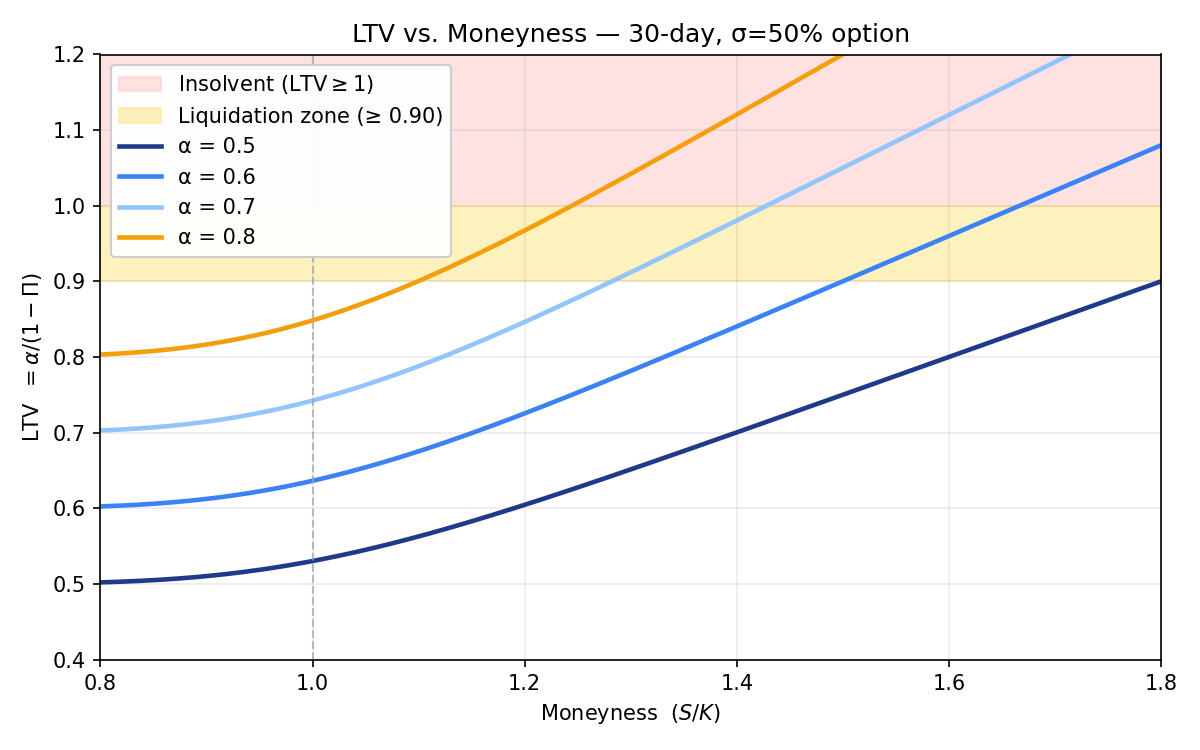
\includegraphics[width=0.45\textwidth]{ltv_curves.png}
  \caption{
    Relative Price of the RT with an estimated OT value; no IV smile, simple option model, strike and underlying invariant, 
    when Moneyness $\geq 1$ $\rightarrow$ ITM. 
    }
  \label{fig:short_price}
\end{figure}

\section{Applications}

\paragraph*{Trading}
The trading interface integrates with Bebop RFQ providing live off-chain pricing with on-chain execution.
Traditional constant-product AMMs ($xy=k$) cannot price the low-volume, asymmetric
distributions that options generate, so the protocol routes order flow through RFQ
market makers who quote signed prices on demand to execute trades. 

OTs can also be auto-minted inside \texttt{transfer()} for seamless JIT delivery, 
allowing market makers to fill an order without holding option inventory ahead of time. 
This provides defragmentation of liquidity, which options trading typically suffers from.

\paragraph*{Default Swaps}
The protocol provides default swaps as insurance for risk management in debt markets.
An oracle or third party can \textbf{unlock} the OT to allow exercise on the
default event.

\paragraph*{Yield Vaults}
Yield vaults can allow LPs to deposit assets to earn yield while Vault curators managing the volatility scalping. 
The strategy is the on-chain analogue of XYLD-style covered-call ETFs, 
but composable where the vault share is itself an ERC20 that downstream protocols can integrate.

\paragraph*{Lending Pool}
For Makers and Traders to write options with capital efficiency they need a pool of lendable assets to borrow from.
The Receipt Troken system allows the Traders to borrow assets from the pool and mint OTs while paying an overnight rate to the lenders.
This is a transformation of the TradFi lending mechanics into onchain options lending mechanics.

\paragraph*{Option Drops Instead of Token Drops}
In TradFi, startup employees vest options and exercise for tax purposes. A similar
mechanic on-chain provides option drops as an alternative to token drops, distributing
upside without giving up immediate sell-pressure protection.

\paragraph*{Compound Options}
A compound option is an option on an option -- a second derivative. The protocol
handles this natively: nothing prevents the OT or RT of one option from being used
as collateral for another option.

\paragraph*{Prediction Markets Derivatives}
Predicion markets can be taken to a derivative level where insurance is available as an option and leverage is available as an option. 
Polymarket is on-chain and provides ERC20 interfaces to their bets. which is a perfect injection into Greek for derivative trading.


\end{document}
